\section{espGG}

No último relatório deste projeto foi encontrado o código fonte da implementação do Grafo de Gabriel
utilizado na biblioteca GGClassification\footcite{https://CRAN.R-project.org/package=GGClassification}
disponível na plataforma CRAN\cite*{CRAN} para a linguagem R\cite*{Rlanguage}. 

A biblioteca foi implementada na linguagem C++ e utiliza uma interface com a linguagem R por meio das bibliotecas Rcpp\footcite{https://github.com/RcppCore/Rcpp}.
O código fonte da biblioteca pode ser encontrado no git:
\url{https://github.com/cran/GGClassification}

Dessa maneira, foi utilizado o código GGClassification como base para o desenvolvimento do projeto espGG, sendo essa a implementação do grafo de Gabriel em um microcontrolador esp32.
Foi também implementado um algoritmo para cálculo de acurácia da predição com os dados de teste.

Utilizando os dados de um dos exemplos disponível na documentação do GGClassification vemos na seguinte imagem os resultados da saída serial do microcontrolador.
Na Figura 1 vemos primeiramente valores finais (cauda) da matrix xTrain. Vemos também os valores de saída yTrain. Os valores de xTest e yTest foram omitidos. 
Em seguida temos avisos de que a função de treinamento (Model) e a função de predição (Predict) foram executadas com sucesso. Logo abaixo vemos o resultado da predição e o valor de acurácia comparado
ao resultado do mesmo algoritmo (GGClassification) em R. 

\begin{figure}[h!]
    \centering
    \label{fig1}
    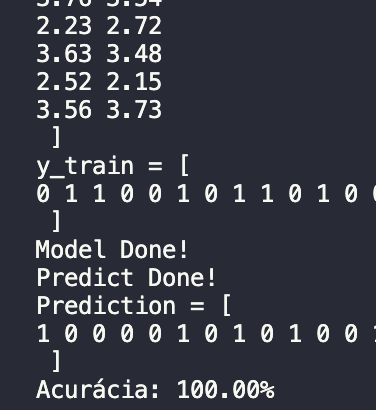
\includegraphics[scale=0.4]{images/espGGserial.png}
    \caption{Resultados do teste realizado.}
\end{figure}

